Successful communication depends on the transfer of reliable information \parencite{endler1993some, searcy2010evolution, hebets2016systems}. In the animal kingdom, information is commonly conveyed by signals which are produced or displayed by one individual to be received by another \parencite{hebets2016systems, searcy2010evolution, seyfarth2010central}. The main purpose of these signals is the prediction of upcoming events and the behavior of other animals in order to make suitable decisions \parencite{endler1993some, seyfarth2010central}. Thereby, signal reliability is a necessity for communication to occur in the first place, as neither the sender would produce signals nor the receiver would respond to them if it were not beneficial for both \parencite{seyfarth2017origin}. Thus, signals conveying reliable information are evolutionary stable even if a sender's and receiver's relationship may be cooperative or competitive \parencite{seyfarth2017origin}. However, the success of communication does not only depend on the signal and its properties itself. Any signal possesses an inherent vagueness that limits its specificity in any situation \parencite{seyfarth2003signalers, seyfarth2017origin}. Therefore, a second necessity for successful communication is contextual information. The context limits the possible interpretations of the information conveyed by the signal, thus increasing its specificity \parencite{seyfarth2017origin}. Hence, both the signal properties and the contextual information frame the communicative event whose success is further determined by the underlying degree of reliability. As such, successful communication is one of the main factors for an animal's survival and reproduction which is why it is the active focus of a wide field of research today.

\subsection{Communication across modalities}

As diverse as the contexts of animal signaling, as diverse are the modalities of the signals themselves. They range from chemical, tactile, and acoustic to visual and even electric, whereby the majority is effectively multimodal \parencite{bradbury1998principles, seyfarth2010central}. One of the most famous examples is the waggle dance of the honeybee \textit{Apis mellifera}, performed to communicate the location of a potent food source to workers in the hive \parencite{von1965tanze, riley2005flight}. As the performance is mainly a visual display it likewise involves scent \parencite{thom2007scent} as well as sound and air flow \parencite{tsujiuchi2007dynamic}. The former is also used by many ant species to indicate a profitable foraging spot. Thereby, the colony is guided by pheromone trails whose compounds are released via specified glands of individual ants \parencite{sudd1959interaction, david2009trail}. Another type of dance besides the honeybee's can be found in the peacock spider \textit{Maratus volans}. However, instead of dancing their way to a promising food source, male peacock spiders perform to impress females to find a partner to mate with \parencite{girard2011multi}. Not only because of the complex motion patterns and ornament displays but likewise owing to the vibratory signals emitted by the males, the peacock spider dance probably marks one of the most impressing communication signals in the animal kingdom \parencite{girard2011multi}. Considering the above it appears that invertebrates in general exhibit an interesting repertoire of possibilities to communicate, as there are also cases of facial patterns signifying status and rival assessment in paper wasps \parencite{tibbetts2008visual} as well as vibrational signals transmitted through plants by various insects to convey sex and species information together with directional cues for the potential mate \parencite{virant2004vibrational}.

\vspace{\baselineskip}

Striking examples of communication are also found among vertebrates. In this group, one of the most prevalent ways of conveying information is active vocalization. For instance, various monkey species exhibit an impressing repertoire of different calls, whereby its type depends on the context of the situation \parencite{SCHLENKER2016894}. One prominent example are the predator-specific calls in vervet monkeys indicating an attack by either a leopard, snake, or eagle \parencite{seyfarth1980}. Moreover, many species are likewise capable of communicating via facial and bodily gestures, which has for example been found in squirrel monkeys \parencite{anderson2010flexibility}, and chimpanzees \parencite{hobaiter2011gestural}. However, not only our closest ancestors but songbirds also use their voices through inter-individual contact. Especially during courtship, males like to show off their song repertoire to convey their qualities to a potential female mate and to repel competitors \parencite{kroodsma1991function, byers2009female}. Whereas a large fraction of animal communication can hardly be overheard, there is an equally large part escaping from human perception. Rodents, for example, emit calls with frequencies way above \SI{20}{\kilo\hertz}: so-called ultrasonic vocalizations (USV) which exceed the human hearing threshold \parencite{wohr2013affective}. These USVs are situation-dependent and differ in frequency. In rats, for instance, three major call types are known: Aversive and appetitive calls emitted by juveniles and adults, and pup calls indicating social isolation \parencite{wohr2013affective, seffer2014pro}. But this is not the only strategy for transferring information in the non-perceivable realm of animal communication. Some groups developed sensory systems enabling them to act both as the sender and receiver of sensory information by using the very same mechanisms \parencite{jonesCommunicationSelfFriends2021}. Such systems are found in pretty distinct species, namely bats \parencite{simmons1979echolocation} and toothed whales \parencite{kamminga1988echolocation}, which rely on echolocation, and weakly-electric fish using electrolocation \parencite{heiligenberg1973electrolocation}. The peculiar thing about these systems is that the animals possessing them actively generate signals to navigate, communicate, and detect prey \parencite{jonesCommunicationSelfFriends2021}. These signals are reflected by objects or other animals and allow for the detection of their properties, distance, and direction. In echolocation, bats and toothed whales emit high-frequency (\SI{20}{\kilo\hertz}) tonal sounds which are produced in the larynx or nose and whose reflections are then gathered by parts of the acoustic system \parencite{schnitzler2003spatial, park2016ultrasonic}. Electrolocation in weakly-electric fish on the other hand is based on the discharge of their electric organ \parencite{heiligenberg1973electrolocation, meyer1987hormone}. They hunt and navigate by perceiving alterations of their electric field caused by other animals or objects \parencite{von1999active, heiligenberg1973electrolocation}. The ability to sense electric fields is not uncommon in aquatic species. Sharks and rays have likewise developed the ability to perceive astoundingly weak electric fields \parencite{kalmijn1971electric}. They use these inputs for prey detection and electrolocation as well, however, they do not produce an electric signal themselves \parencite{kalmijn1971electric, kalmijn1973electro}. The electric eel, for example, is one the few species that is capable of actively producing electricity \parencite{catania2014shocking}. In contrast to weakly-electric fish, however, they do not constantly surround themselves with an electric field, but rather emit a mixture of low- and high-voltage pulses \parencite{catania2014shocking, catania2015electric}. The low-voltage pulses are used for sensing the environment whereas high-voltage pulses serve as a predatory strike to incapacitate prey \parencite{brown1950electric, catania2014shocking, catania2015electric}. The latter can reach strikingly high voltages of up to 600 V \parencite{brown1950electric, catania2014shocking}.

\subsection{Beyond human perception: Weakly electric fish}
As stated above, weakly-electric fish sample their environment by surrounding themselves with an electric field produced by discharging their electric organ. Based on the waveform of the electric organ discharge (EOD), weakly-electric fish are classified into two distinct groups: Wave-type and pulse-type electric fish \parencite{bendaPhysicsElectrosensoryWorlds2020}. Whereas wave-type EODs are characterized by a continuous discharge and a periodic waveform, pulse-type EODs show brief pulses interrupted by intervals of varying length \parencite{bendaPhysicsElectrosensoryWorlds2020}. For the wave-type category, the gymnotiform brown ghost knifefish \textit{Apteronotus leptorhynchus} is one of the best and most extensively studied species \parencite{zupanc1993evoked, meyer1987hormone, malerAtlasBrainElectric1991, hupeEffectDifferenceFrequency2008, englerSpontaneousModulationsElectric2000a, hagedornCourtSparkElectric1985a, dunlapHormonalBodySize2002}. Its EOD has a quasi-sinusoidal waveform and typically lies in a frequency range of \SIrange{600}{1000}{\hertz} (Fig. \ref{fig:Electric fields}B) \parencite{zupanc1993evoked, zakonEODModulationsBrown2002a}. Moreover, \textit{A. leptorhynchus} shows a sexual dimorphism in EOD frequency (EOD$f$) with females having a lower EOD$f$ ($<$ \SI{750}{\hertz}) than male individuals ($>$ \SI{750}{\hertz}) \parencite{meyer1987hormone, zakonEODModulationsBrown2002a}. Communication between two individuals occurs first and foremost because of the physical properties of the electric field. When interacting, the electric fields of two fish superimpose and result in amplitude modulation (AM), also called beat (Fig. \ref{fig:Electric fields}A \& D) \parencite{zupanc1993evoked, walzNeuroethologyElectrocommunicationHow2013, benda2005spike, bendaPhysicsElectrosensoryWorlds2020}. That is, by interacting with another individual, one fish perceives its own EOD being modulated by another electric field. The resulting beat has a specific frequency which is given by the frequency difference of the two interacting fish \parencite{benda2005spike, walzNeuroethologyElectrocommunicationHow2013, bendaPhysicsElectrosensoryWorlds2020}. Because of the frequency dimorphism in \textit{A. leptorhynchus}, this allows for a passive exchange of information since the beat frequency concomitantly transfers the gender relation of the fish. Simply speaking, the greater the beat frequency, the more likely it is that the other fish is of the opposite gender. However, \textit{A. leptorhynchus} is likewise capable of producing active communication signals. One of the most extensively studied are chirps \parencite{zupanc1993evoked, zakonEODModulationsBrown2002a, englerSpontaneousModulationsElectric2000a, hupeElectrocommunicationSignalsFree2009, obotiWhyBrownGhost2022, dunlapDiversityStructureElectrocommunication2003}. Chirps are transient frequency modulations that, depending on the type, are characterized by a duration of ten to a few hundred milliseconds and an increase of EOD$f$ up to several hundred Hertz (Fig. \ref{fig:introplot}, red track) \parencite{bendaPhysicsElectrosensoryWorlds2020, zupanc1993evoked, engler2001differential, zakonEODModulationsBrown2002a}. They have been shown to play a role in courtship and the synchronization of spawning \parencite{hagedornCourtSparkElectric1985a, henningerStatisticsNaturalCommunication2018}, but are also associated with aggressive encounters \parencite{triefenbachChangesSignallingAgonistic2008b}, where they are suggested to serve as a submissive signal \parencite{walzNeuroethologyElectrocommunicationHow2013, henningerStatisticsNaturalCommunication2018}. However, because of the various contexts in which chirps are emitted, their function is still an ongoing debate \parencite{obotiWhyBrownGhost2022}.

\begin{figure}[H]
    \centering
    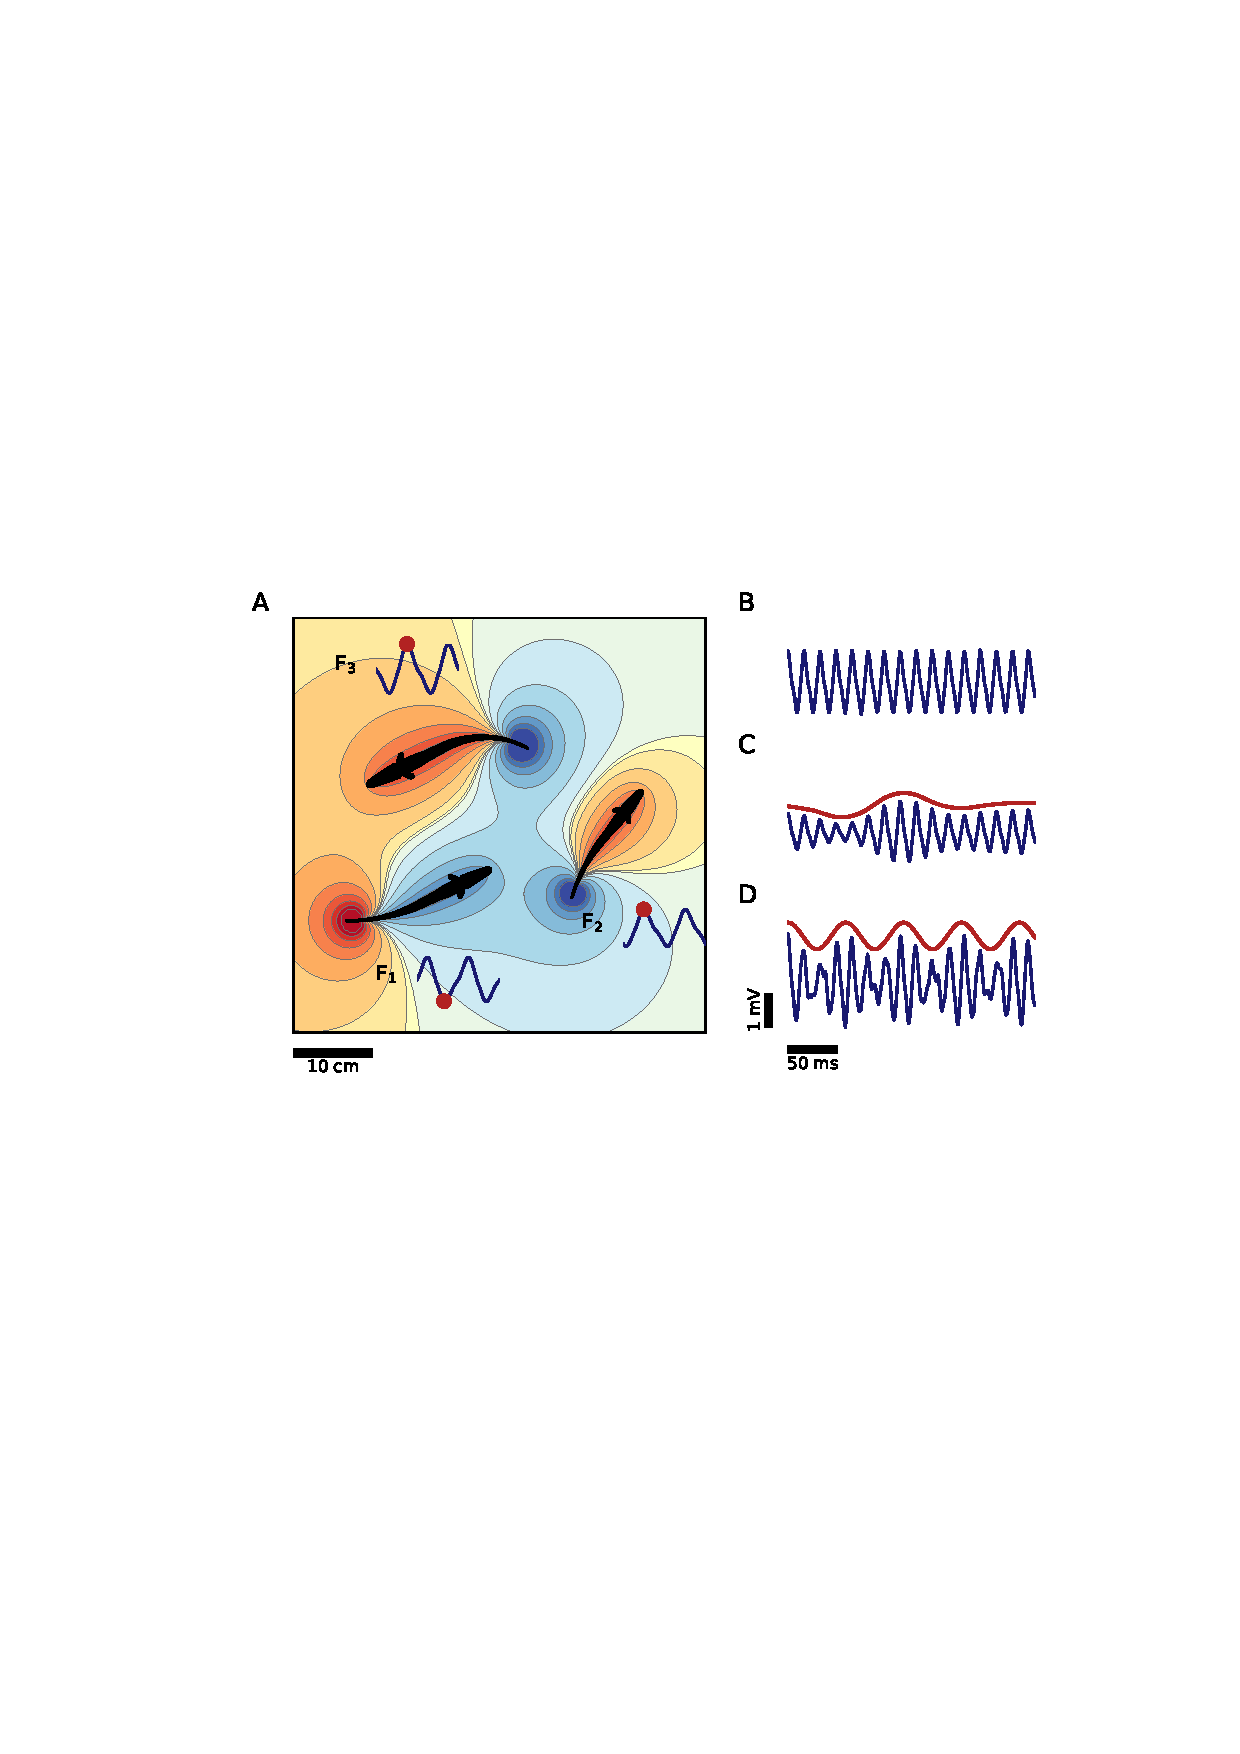
\includegraphics[width=0.7\linewidth]{figures/Fishies_cropped.pdf}
    \mycaption{Properties of the electric field in weakly-electric fish}{\textbf{A:} The fish surround themselves with a bipolar electric field. The superposition of electric fields alters their spatial properties. Thereby, the phase of the EOD influences the extend and direction of the electric field of each fish (red marker in EOD waveform). \textbf{B:} Quasi-sinusoidal waveform of the EOD of a single wave-type electric fish. \textbf{C:} Amplitude modulations (AM) of an individual fish recorded by external electrodes. The AM is caused by the movements of the fish relative to the recording electrodes. \textbf{D:} Amplitude modulation or beat caused by the superposition of two electric fields. The frequency of the beat is given by the difference in frequency between the individual fish (Figure from \cite{raab2022social}).}
    \label{fig:Electric fields}
\end{figure}

\subsection{The problem of detection}
For the exploration of the chirp function, two requirements have to be met. First, chirps need to be recorded to be analyzed in the first place. Secondly, the analysis depends on the ability to detect chirps in the recordings. Optimally, the method fulfilling these two requirements is suited for deployment in laboratory settings as well as in the field. Chirp recording is the least problematic part. As chirps alter the EOD$f$, they can readily be recorded by a pair of electrodes placed in the vicinity of the fish \parencite{bendaPhysicsElectrosensoryWorlds2020}. A common approach in laboratory settings is to simulate a conspecific with a pair of electrodes which should cause the recorded individual to chirp. These can then be recorded with a second pair of electrodes \parencite{zupanc1993evoked, hagedornCourtSparkElectric1985a, dunlapDiversityStructureElectrocommunication2003, englerSpontaneousModulationsElectric2000a}. However, the laboratory does not reflect the natural habitat of the animals since the behavioral context of chirps emitted in the wild is highly variable \parencite{henningerStatisticsNaturalCommunication2018}. Thus, there is a need of recording fish in their natural habitat while freely behaving and interacting with each other. This is why recently, research is more and more shifted to the field \parencite{henningerStatisticsNaturalCommunication2018, fugere2011electrical, zubizarreta2020seasonal}. With this increasing change in research approach, new methods that allow for the recording of multiple fish in the wild were required. One approach was developed by \textcite{henningerStatisticsNaturalCommunication2018} and successfully tested in Panama, where the authors simultaneously recorded multiple individuals of four species of weakly-electric fish. They used a grid-like array of at least 54 electrodes which was submerged at the cut bank side of a stream. Later, a refined version of the grid was applied for further recordings in Colombia \parencite{raab2022AdvancesNoninvasiveTracking}. As such, the recording problem has been solved for the laboratory as well as the natural setting. The detection of chirps, however, turned out to be the bigger problem. As part of successful detection, it is required to correctly identify the chirp in the EOD track as well as assign the individual chirp to the correct animal. This is particularly difficult in recordings of multiple fish because the detection of a chirp implies that the underlying EOD$f$ is tracked for every animal. One approach for the analysis of electric signals in weakly-electric fish are spectrograms (Fig. \ref{fig:introplot}). Since chirps are very fast changes in the EOD$f$, a sufficiently high resolution in the time domain is necessary to resolve them. But, an increase of the resolution in time is accompanied by a resolution decrease in the frequency domain, which renders the distinction of the EOD$f$s of the chirping fish impossible. Given the situation of two fish with a similar EOD$f$, and the individual with the lower frequency emitting a chirp, it is unfeasible to assign the chirp to the correct individual by only using the spectrogram. Thus, chirp detection is surely not a trivial problem. \textcite{raab2022AdvancesNoninvasiveTracking}, based on previous work by \textcite{henningerTrackingActivityPatterns2020}, developed an algorithm that solves one part of the issue. It is capable of extracting EOD tracks by using both the EOD$f$ in the spectrogram as well as the spatial distribution of EOD power across electrodes \parencite{raab2022AdvancesNoninvasiveTracking}. This way, it is possible to obtain the EOD track of individual fish in recordings with multiple fish in space and time (Fig. \ref{fig:introplot}). Only with this groundwork, it is achievable to detect chirps in the first place. 

\vspace{\baselineskip}

To overcome the remaining problem of chirp assignment, we refined previous work on this issue \parencite{henningerStatisticsNaturalCommunication2018}. In the following, we describe and test the first draft of a chirp detection algorithm capable of assigning chirps to individual fish in recordings with multiple animals. Our approach was to include a dynamic filter that searches for a frequency range between the individual EOD$f$'s free of interference. In a second step, we tested the algorithm with a data set obtained by \textcite{raabElectrocommunicationSignalsIndicate2021}. Thereby, individuals of the species \textit{Apteronotus leptorhynchus} were recorded while competing for a superior shelter in dyads. We were able to detect 25766 chirps in this data set alone and analyzed the context in which they were emitted. Thereby, we could not fully replicate suggestions for chirp function from the literature. However, some of our results indicate the association of chirps with a specific type of event during aggressive encounters.

\begin{figure}[H]
    \centering
    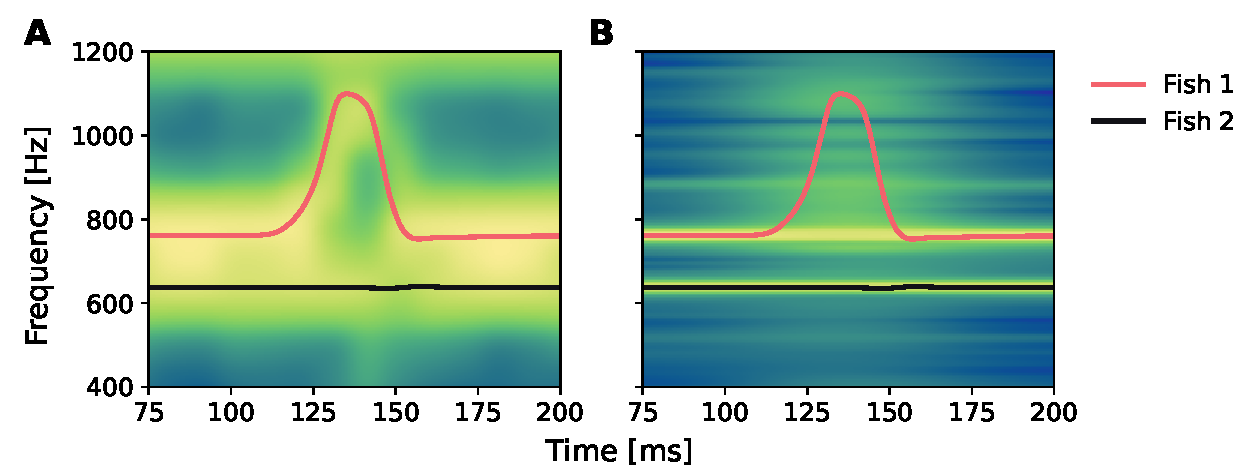
\includegraphics[width=1\linewidth]{figures/introplot.pdf}

    \mycaption{Spectrogram of signal containing the EODs of two fish.}{The line plots indicate the instantaneous frequency of the respective individual, which we obtained by filtering the signal around its frequency component. \textbf{A:} Fish 1 produces a chirp that is visible by the frequency excursion in the instantaneous frequency and spectrogram if the frequency resolution is sufficient (NFFT=133.3, 20\% overlap). \textbf{B:} If the frequency resolution is lower, fish can be distinguished in the spectrogram, but chirp detection and assignment are not reliable (NFFT=1333.3, 20\% overlap). }
    \label{fig:introplot}
\end{figure}

\todo[inline, color=orange]{Bilder von Lepto und seiner EOD waveform?}
\todo[inline, color=orange]{Messy in-text Quellen}
\todo[inline, color=orange]{Messy references Quellen}
